%!TEX root = ../Main.tex

\chapter{Exercise 3.5}
\textbf{Implement a model that demonstrates a system design that transfer data at the TLM level
refined to BCAM level. Use the sc\_fifo to model communication at the TLM level and refine it to
BCAM using adapters as inspiration study the example project SmartPitchDetector (InAdapter.h
and OutAdapter.h). Here a master sends data to a slave using a sc\_fifo and an adapter that
converts to the bus cycle accurate interface on the receiving slave. Use the model from exercise
3.4 for the interface at the Avalon-ST sink interface for the slave as illustrated below}

\section{Master.cpp}
In this exercise the master sends 10 integers to the slave. The code for the master can be seen below.
\begin{lstlisting}
void Master::MasterThread(void)
{
	// send the values in the array
	int i = 0;
	while(i<10)
	{
		cout << "Master writing: " << dataToSend[i] << endl;
		data_out.write(dataToSend[i]);
		i++;
	}
}
\end{lstlisting}


\section{Slave.cpp}
The slave behaves almost as in exercise 3.4 but without the ability to write to a text file. The code for the slave can be seen below.

\begin{lstlisting}
void Slave::SlaveThread(void)
{
	// Initial state of "ready".
	ready.write(false);
	
	// Simulate ready going low for 3 cycles, then high for 3 cycles, etc..
	while (1)
	{
		// read new data if any valid data
		if (valid.read())
		{
			data_read = data.read();
			data_read_array[array_index] = data_read;
			array_index++;
			cout << "Slave received data: " << data_read << endl;
		}
		
		// Make sure that slave is ready for 3 cycles, then not ready for 3 cycles.
		if (state_counter < 3)
		{
			ready.write(true);
		}
		else
		{
			ready.write(false);
		}
		state_counter++;
		state_counter = state_counter % 6;
		
		wait(clk.posedge_event());
	}
};
\end{lstlisting}


\section{Top.cpp}
The Top.cpp files show how the adaptor is in between the master and slave. On the figure below the code show how this is done.


\begin{lstlisting}
TOP::TOP(sc_module_name nm) :
clock("clock", sc_time(20, SC_NS))
{
	// Set reset to false
	reset.write(false);
	
	// Create instance of Master, Slave and InAdapter
	slave = new Slave("slave");
	master = new Master("master");
	inAdapter = new InAdapter<sc_int<DATA_BITS>>("inAdapter");
	
	// Connect inputs and outputs of Slave to signals.
	slave->ready(ready);
	slave->valid(valid);
	slave->clk(clock);
	slave->data(data);
	slave->error(error);
	slave->channel(channel);
	
	// Connect master to fifo.
	master->data_out(*inAdapter);
	
	// Connect adaptor to slave
	inAdapter->data(data);
	inAdapter->ready(ready);
	inAdapter->valid(valid);
	inAdapter->clk(clock);
	inAdapter->error(error);
	inAdapter->channel(channel);
	inAdapter->reset(reset);
	
	//Tracefile configuration
	sc_trace_file *tracefile;
	tracefile = sc_create_vcd_trace_file("Avalon_Streaming_Bus");
	if (!tracefile) cout << "Could not create trace file." << endl;
	tracefile->set_time_unit(1, SC_NS); // Resolution of trace file = 1ns
	sc_trace(tracefile, clock, "clock");
	sc_trace(tracefile, ready, "ready");
	sc_trace(tracefile, valid, "valid");
	sc_trace(tracefile, data, "data");
	sc_trace(tracefile, error, "error");
	sc_trace(tracefile, channel, "channel");

}
\end{lstlisting}

\section{InAdaptor.cpp}
The adaptor makes sure that you get a cycle accurate model when using TLM style communication, like the sc\_fifo. The code for the adaptor can be seen below.

\begin{lstlisting}
template <class T>
class InAdapter : public sc_fifo_out_if <T>, public sc_module
{
	public:
	// Clock and reset
	sc_in_clk clk; // Clock
	sc_in<bool> reset; // Reset
	
	// Handshake ports for ST bus
	sc_in<bool> ready; // Ready signal
	sc_out<bool> valid; // Valid signal
	
	// Channel, error and data ports ST bus
	sc_out<sc_int<CHANNEL_BITS> > channel;
	sc_out<sc_int<ERROR_BITS> > error;
	sc_out<sc_int<DATA_BITS> > data;
	
	void write(const T & value)
	{
		cout << "InAdapter: write(" << value << ")" << endl;
		
		// If 'reset' is high, just wait.
		if (reset == false)
		{
			// Output sample data on negative edge of clock
			
			// Wait until ready is high
			while (ready == false)
			wait(clk.posedge_event());
			
			// Wait 1 clock cycle to simulate 1 clock cycle delay.
			// wait(clk.posedge_event());
			
			// Write "high" to valid, indicating that data is being written.
			valid.write(true);
			
			// Write data
			data.write(value);
			
			// Write channel and error info
			channel.write(0); // Channel number
			error.write(0); // Error
			
			// Wait one clock cycle, then indicate that data is not being written anymore
			wait(clk.posedge_event());
			valid.write(false);
		}
		else wait(clk.posedge_event());
	}
	
	
	InAdapter(sc_module_name name_)
	: sc_module(name_)
	{ }
	private:
	bool nb_write(const T & data)
	{
	SC_REPORT_FATAL("/InAdapter", "Called nb_write()");
	return false;
	}
	virtual int num_free() const
	{
	SC_REPORT_FATAL("/InAdapter", "Called num_free()");
	return 0;
	}
	virtual const sc_event& data_read_event() const
	{
	SC_REPORT_FATAL("/InAdapter", "Called data_read_event()");
	return *new sc_event;
	}
};
\end{lstlisting}

A tracefile has also been generated for this exercise. It is almost identical to the tracefile from exercise 3.4, which means the adaptor works as intended and the model is cycle accurate. The tracefile can be seen below.

\begin{figure}[H]
	\centering
	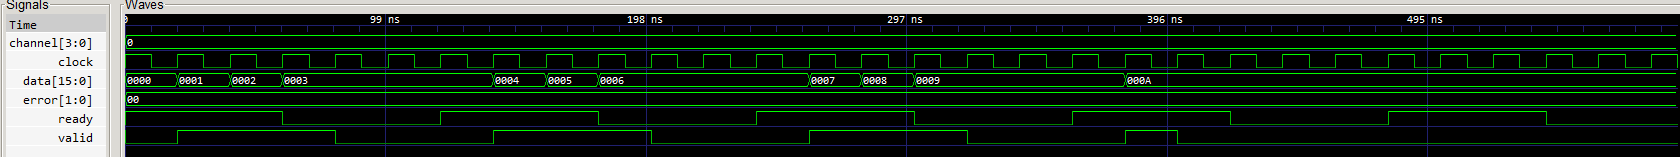
\includegraphics[width=\textwidth]{Images/GTK_3_5.png}
	\caption{A screenshot of GTK viewer}
	\label{fig:GTK_Viewer2}
\end{figure}

In the console windows it can be seen how the master sends data to the adaptor which redirects the data to the slave.

\begin{figure}[H]
	\centering
	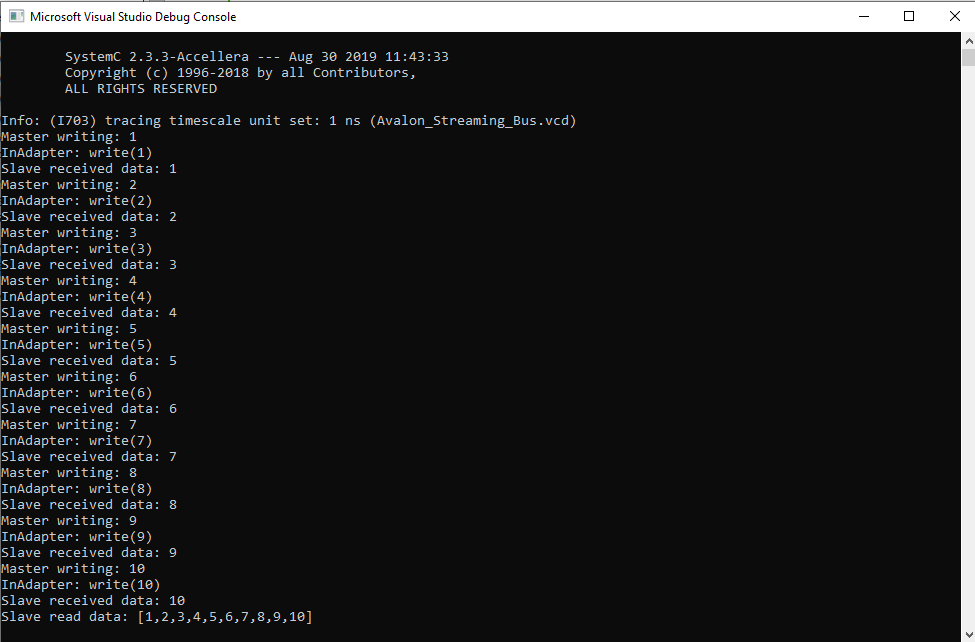
\includegraphics[width=\textwidth]{Images/ConsoleWindow3_5.png}
	\caption{A screenshot of the console}
	\label{fig:ConsoleWindow}
\end{figure}

 